\chapter{Introducción específica} % Main chapter title

\label{Chapter2}

\textbf{AGREGAR TEXTO DESCRIPTIVO SOBRE LA INTRO ESPECIFICA}

%----------------------------------------------------------------------------------------
\section{Protocolos de comununicación utilizados}

  Comenzar escribiendo que aqui se detallaran los protocolos utilizados segun el modelo TCP/IP y hablar sobre el diagrama    

  AGREGAR UNA IMAGEN CON LOS 3 ENTES INTERCONECTADOS BAJO EL MODELO TCP/IP 
        Nucleo F429ZI Board <----> Dedicated Server <----> Web Client


\subsection{Protocolos de comunicación}

De los modelos \textit{stack IoT} y \textit{lwIP} \citep{lwip}, basados en el stack \textit{TCP/IP} \citep{tcpip}, se emplean los siguientes protocolos de comunicación tal como se puede observar en la tabla \ref{tab:capa_protocolo}. 


\begin{table}[h]
\centering
\caption{Protocolos de comunicación utilizados en cada capa del \textit{stack TCP/IP}}
\label{tab:capa_protocolo}
\begin{tabular}{|c|c|}
\hline
\textbf{Capa} & \textbf{Protocolo} \\ \cline{1-2}
Capa de Aplicación & HTTP \citep{http}, DHCP \citep{dhcp} y MQTT \citep{mqtt} \\ \cline{1-2}
Capa de Transporte & UDP \citep{udp} \\ \cline{1-2}
Capa de Red & IPv4 \citep{ipv4}, ARP \citep{arp} \\ \cline{1-2}
Capa de Enlace de Datos & Ethernet \citep{ethernet} \\ \cline{1-2}
\end{tabular}
\end{table}

Cabe destacar que ambos modelos se encuentran diseñados para sistemas con recursos limitados y buscan garantizar una correcta comunicación entre los dispositivos conectados en la red.


%----------------------------------------------------------------------------------------
\section{Tecnologías \textit{full-stack}}

A partir de los modelos más relevantes que se encuentran establecidos para el desarrollo e implementación de aplicaciones de software se consideran el \textit{stack web} y el \textit{stack IoT}, tal como se puede ver en la figura \ref{fig:diagBloques}. A pesar de las similitudes entre ambos, en la aplicación el \textit{stack web} emplea el protocolo \textit{HTTP} mientras que el \textit{stack IoT} utiliza el protocolo \textit{MQTT}; siendo este último el más adecuado para escenarios donde son limitados los recursos como el ancho de banda y el consumo de energía.

En especial, el protocolo \textit{MQTT} dispone de mensajes más livianos y además es posible transmitir y/o recibir datos en formato binario sin la necesidad de una codificación previa. También, este protocolo permite asignar niveles de calidad de servicio (\textit{QoS} \citep{ibm-qos}) a los mensajes transmitidos, resultando una característica primordial en aplicaciones donde la probabilidad de pérdidas de paquetes es considerable.


\begin{figure}[htpb]
  \centering 
  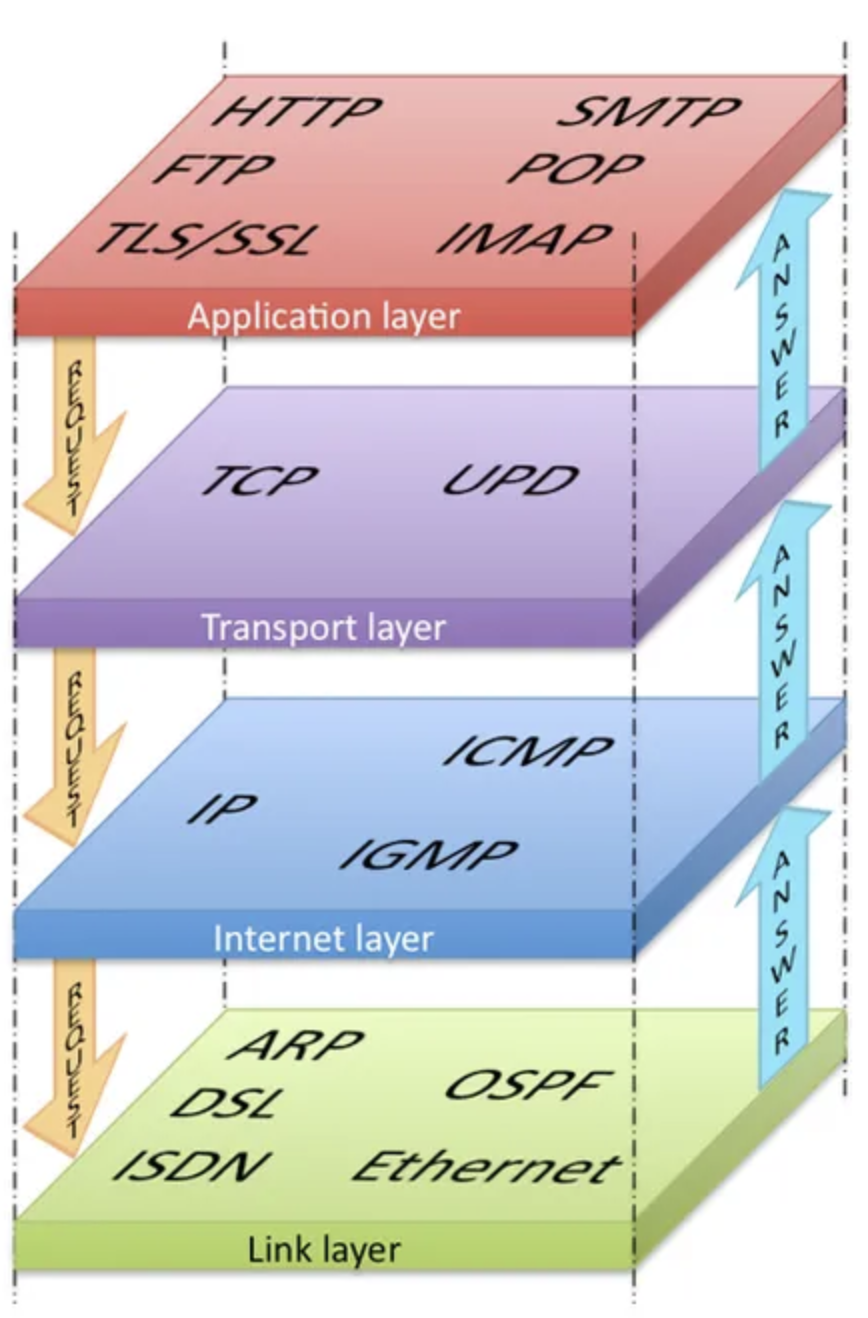
\includegraphics[width=.4\textwidth]{Figures/tcp-ip-stack.png}
  \caption{Arquitectura de la pila de protocolos \textit{TCP/IP}.}
  \label{fig:diagBloques}
\end{figure}


\subsection{Tecnologías del \textit{front-end}}

\subsubsection{TypeScript}

\textit{TypeScript} \citep{typescript} es una extensión de código abierto de \textit{JavaScript} que agrega tipos estáticos opcionales y características de programación orientada a objetos avanzadas, lo que permite una mayor seguridad y mantenibilidad en el código. 


\subsubsection{React}

\textit{React} \citep{react} es una biblioteca de \textit{JavaScript} para construir una interfaz de usuario reutilizable e interactiva, desarrollada por \textit{Facebook} y ampliamente utilizada en el desarrollo web. Usa un enfoque basado en componentes y el \textit{DOM} virtual para mejorar el rendimiento y es altamente integrable con otras bibliotecas y frameworks.


\subsubsection{Parcel}

Parcel \citep{parcel} es una herramienta de construcción de código abierto con una estrategia de cero configuración que optimiza y empaqueta módulos de JavaScript y otros archivos. En particular, mejora significativamente el flujo de trabajo del desarrollador al ser rápido, fácil de usar y altamente personalizable.


\subsubsection{Apollo GraphQL}

\textit{Apollo GraphQL} \citep{apollo-graphql} es una plataforma de código abierto para el desarrollo de aplicaciones \textit{GraphQL}, con una amplia gama de herramientas y servicios para construir y mantener aplicaciones \textit{GraphQL} de manera efectiva, ofreciendo una administración de caché y una amplia compatibilidad con diferentes \textit{frameworks} y tecnologías.


\subsubsection{Material UI}

\textit{Material UI} \citep{material-ui} es una biblioteca de componentes de interfaz de usuario de código abierto basada en Material Design de Google, ofrece componentes preconstruidos altamente personalizados y una amplia compatibilidad con diferentes tecnologías y frameworks para construir aplicaciones web modernas y atractivas.


\subsubsection{JWT Decode}

\textit{JWT Decode} \citep{jwt-decode} es una biblioteca \textit{JavaScript} que decodifica \textit{tokens JWT}, con características útiles como validación de tokens y verificación de firma. Se integra fácilmente en diferentes \textit{frameworks} de \textit{JavaScript} como \textit{React} y \textit{Angular}.


%----------------------------------------------------------------------------------------
\subsection{Tecnologías del \textit{backend}}


\subsubsection{Kotlin}

\textit{Kotlin} \citep{kotlin} es un lenguaje de programación de tipado estático que puede correr sobre la máquina virtual de \textit{Java} y ser compilado en \textit{JavaScript} y \textit{LLVM}. También ofrece interoperabilidad con \textit{Java}, programación funcional, orientación a objetos y manejo de nulos seguro, lo que ha llevado a su popularidad debido a su facilidad de uso y legibilidad.


\subsubsection{Ktor}

\textit{Ktor} \citep{ktor} es un \textit{framework} web de \textit{Kotlin} que permite crear aplicaciones web y \textit{API REST} de manera fácil y eficiente, con un enfoque en la programación funcional. \textit{Ktor} es altamente modular y personalizable, lo que significa que los desarrolladores pueden seleccionar solo los componentes que necesitan para su aplicación, reduciendo así la complejidad y el tamaño del código. 


\subsubsection{Kafka}

\textit{Kafka} \citep{kafka} es una plataforma de \textit{streaming} de datos que permite a las aplicaciones enviar y recibir datos en tiempo real. Se encuentra basada en el modelo de publicación/suscripción, se caracteriza por su alta velocidad y rendimiento, haciéndola ideal para aplicaciones que necesitan procesar grandes cantidades de datos en tiempo real.


\newpage
\subsubsection{Hasura}

\textit{Hasura} \citep{hasura} es una plataforma sin servidor que permite a los desarrolladores crear y escalar aplicaciones con \textit{GraphQL} rápidamente. Ofrece seguridad de extremo a extremo y se integra fácilmente con diferentes bases de datos para generar automáticamente una \textit{API} de \textit{GraphQL}.

\subsubsection{PostgreSQL}

\textit{PostgreSQL} \citep{postgresql} es un sistema de gestión de bases de datos de código abierto y gratuito, conocido por su fiabilidad, escalabilidad y seguridad. Ofrece soporte para transacciones \textit{ACID}, integración con lenguajes de programación populares y una amplia variedad de herramientas y extensiones.


\subsubsection{Mosquitto Broker}

\textit{Mosquitto} \citep{mosquitto} es un \textit{broker} \textit{MQTT} de código abierto utilizado en \textit{IoT} para transmitir mensajes entre dispositivos. Es popular por su escalabilidad, facilidad de uso y características de seguridad.


%----------------------------------------------------------------------------------------
\subsection{Tecnologías del \textit{firmware}}


\subsubsection{C lang}

C \citep{c-lang} es un lenguaje de programación estructurado y de propósito general, ampliamente utilizado en sistemas operativos, aplicaciones de bajo nivel y dispositivos embebidos. Su sintaxis simple y directa permite escribir código claro y legible, y ofrece gran control sobre la memoria y acceso directo al hardware.


\subsubsection{FreeRTOS}

\textit{FreeRTOS} \citep{free-rtos} es un \textit{RTOS} de código abierto y gratuito que controla sistemas embebidos y microcontroladores, utilizado en control industrial, automoción y electrónica de consumo, con capacidad de rendimiento confiable y predecible. Es altamente portátil y ofrece gestión de tareas, semáforos, colas y temporizadores para sistemas complejos y eficientes en recursos.


\subsubsection{Paho MQTT \textit{client}}

\textit{Paho} \citep{paho-mqtt} es una biblioteca que desarrolla un cliente \textit{MQTT} de código abierto que se utiliza para conectar aplicaciones a un \textit{broker} \textit{MQTT}. \textit{Paho} es compatible con una amplia variedad de plataformas y lenguajes de programación, brinda una \textit{API} sencilla para publicar y suscribir mensajes. Es ampliamente utilizado en aplicaciones de \textit{IoT} y \textit{M2M} para la transmisión eficiente de datos.


%----------------------------------------------------------------------------------------
\subsection{Herramientas utilizadas}


\subsubsection{Docker}

\textit{Docker} \citep{docker} es una plataforma de software que permite a los desarrolladores crear, desplegar y ejecutar aplicaciones en contenedores. Estos contenedores permiten que las aplicaciones se ejecuten de manera aislada del sistema operativo y otras aplicaciones, lo que facilita su portabilidad y escalabilidad. 


\subsubsection{Docker Compose}

\textit{Docker Compose} \citep{docker-compose} es una herramienta que permite definir y ejecutar aplicaciones de múltiples contenedores \textit{Docker}. Permite a los desarrolladores especificar los servicios y la configuración de cada contenedor en un archivo \textit{YAML}a \citep{yaml} para simplificar la creación, ejecución y gestión de aplicaciones complejas. 


\subsubsection{Redpanda}

\textit{Redpanda} \citep{redpanda} es una plataforma de \textit{streaming} de datos distribuida y de alto rendimiento que combina las funcionalidades de \textit{Kafka} y \textit{Redis}. Es una solución escalable y confiable para el procesamiento de datos en tiempo real en entornos empresariales, y es compatible con una amplia variedad de casos de uso, desde el análisis de datos hasta la inteligencia artificial y el aprendizaje automático.


\subsubsection{Git}

\textit{Git} \citep{git} es un sistema de control de versiones distribuido que se utiliza para rastrear los cambios en el código fuente de un proyecto de software. Permite a los desarrolladores trabajar en colaboración en el mismo código fuente y hacer un seguimiento de las diferentes versiones y ramas del proyecto. 


\subsubsection{MQTT.fx}

\textit{MQTT.fx} \citep{mqtt-fx} es una herramienta de escritorio de código abierto que se utiliza para probar y depurar conexiones \textit{MQTT}. Ofrece una interfaz gráfica de usuario fácil de usar para interactuar con \textit{brokers MQTT} y suscribirse a temas y mensajes. \textit{MQTT.fx} es compatible con una variedad de características de seguridad, como \textit{TLS/SSL} y autenticación, lo que lo hace adecuado para su uso en entornos de producción.


\subsubsection{CLion}

\textit{CLion} \citep{clion} es un entorno de desarrollo integrado (\textit{IDE}) para programar en C y C++ que proporciona herramientas para la edición de código, depuración, refactorización y gestión de proyectos. Es conocido por su alta capacidad de análisis estático de código, lo que permite a los desarrolladores encontrar errores de forma eficiente.


\subsubsection{Wireshark}

\textit{Wireshark} \citep{wireshark} es una herramienta de análisis de redes de código abierto y gratuita, utilizada para capturar y analizar paquetes de datos en tiempo real. Permite examinar el tráfico de red para identificar problemas de rendimiento, seguridad y configuración; siendo compatible con una amplia variedad de protocolos de red.


\subsubsection{Herramientas del navegador de internet}

Las herramientas del navegador de internet son características incorporadas que permiten a los usuarios analizar y modificar elementos de una página web, como su estructura \textit{HTML}, \textit{CSS} y \textit{JavaScript}. Algunas herramientas comunes incluyen la consola de desarrollador, el inspector de elementos, el depurador de \textit{JavaScript} y el analizador de red, que ayudan a los desarrolladores a depurar problemas y mejorar la calidad de sus sitios web.


\subsubsection{JTAG}

\textit{JTAG} (\textit{Joint Test Action Group}) \citep{jtag} es un estándar para la depuración y programación de dispositivos electrónicos. Permite acceder a los pines de prueba de un dispositivo para realizar pruebas de hardware y depuración a nivel de circuito. \textit{JTAG} se ha convertido en un estándar común para la depuración y programación de dispositivos, y muchas herramientas de desarrollo de software y hardware lo admiten.


\subsubsection{ST-Link}

\textit{ST-Link} \citep{st-link} es una herramienta de programación y depuración de microcontroladores fabricada por \textit{STMicroelectronics}. Se utiliza para programar y depurar microcontroladores \textit{STM32} y otros dispositivos compatibles con \textit{JTAG} o \textit{SWD}. La herramienta se conecta al ordenador mediante \textit{USB} y se puede usar con una variedad de entornos de desarrollo integrados (\textit{IDE}) y herramientas de depuración. 


\subsubsection{STM32CubeMX}

\textit{STM32CubeMX} \citep{stm32-cubemx} es una herramienta de configuración gráfica para dispositivos \textit{STM32} que permite a los desarrolladores generar automáticamente código inicial para su proyecto. Ofrece una interfaz de usuario intuitiva que simplifica la configuración de periféricos y pines, además, admite una variedad de opciones de generación de código. 


\subsubsection{STM32CubeProgrammer}

\textit{STM32CubeProgrammer} \citep{stm32-cubeprogrammer} es una herramienta de programación y actualización de firmware para dispositivos \textit{STM32} que permite programar y depurar dispositivos \textit{STM32}, así como actualizar su firmware en campo. Es compatible con una variedad de interfaces de programación, como \textit{JTAG}, \textit{SWD} y \textit{UART}, también, es fácil de usar gracias a su interfaz gráfica de usuario. 



